\documentclass[11pt,a4paper,english]{article}
  \usepackage[latin1]{inputenc}
  \usepackage{amsmath,amsfonts,amssymb}
  \usepackage{enumitem}
  \usepackage{fullpage}
  \usepackage{graphicx}
  \usepackage{tabto}
  \usepackage{etoolbox}
  \usepackage{hyperref}
  \usepackage{minted}
  \usepackage{parskip}
  \usepackage[font=small,labelfont=bf]{caption}
  \renewcommand{\labelenumii}{\theenumii}
  \renewcommand{\theenumii}{\theenumi.\arabic{enumii}.}

  \title{Algorithmic Methods of Data Mining - Assignment 2}
  \author{Maksad Donayorov}

  \begin{document}
    \maketitle
    \definecolor{bg}{rgb}{0.95,0.95,0.95}

    \begin{enumerate}
      \item \textbf{Problem:} \textit{Bag of words:}

      \item \textbf{Problem:} $\mathcal{O}(\log{w}\ \log{n})$: \\
        Before analyzing the complexity and responding to the question it could be nice to see an algorithm that finds the $max$ number in an array. Such algorithm can be easily written in python, that gives us a clear picture of how the computation is done:
        \begin{minted}[bgcolor=bg,linenos,fontsize=\small,autogobble]{js}
          def get_max(arr):
            max_num = -1
            for el in arr:
              if max_num < el:
                max_num = el
            return max_num
        \end{minted}

        The best case for finding the $max$ element is when the first element is bigger than all of the other elements of $X$, which has complexity of $\mathcal{O}(1)$. And the worst case is when the last element is the largest and all the consecutive numbers proceed from small to large. This case has a complexity of $\mathcal{O}(n)$. The tricky part is the average case, where we have to compute the complexity for \textit{the number of times that max is assigned to an element}.

        Assuming that $X[1,2,3...m]$ is drawn independently and uniformly at random from the interval $(0,1)$, the expected value will be:
        \begin{align*}
          E[x] = \sum\limits_{i=1}^{m} Pr(X_i)
        \end{align*}
        Where $Pr(X_i)$ is the probability of the \textit{i-th} element being the $max$ element in $X[1,2,3...m]$. To have a better intuition of what could be the probability of \textit{i-th} element we can have a look at different size of $m$:
        \begin{align*}
          Pr(x_1) & = 1 \\
          Pr(x_2) & = \frac{1}{2} \\
          Pr(x_3) & = \frac{1}{3} \\
                  & ... \\
          Pr(x_m) & = \frac{1}{m} \\
        \end{align*}
        Looking at this we can infer that the expected value can be calculated as:
        \begin{align*}
          E[x] = 1 + \frac{1}{2} + \frac{1}{3} + ... + \frac{1}{m} = \sum\limits_{i=1}^{m}{\frac{1}{i}} \approx \log{m}
        \end{align*}
        Consequently, we can conclude that $max = X[i]$ will be executed $\mathcal{O}(\log m)$ times, on expectation.

        \begin{center}
          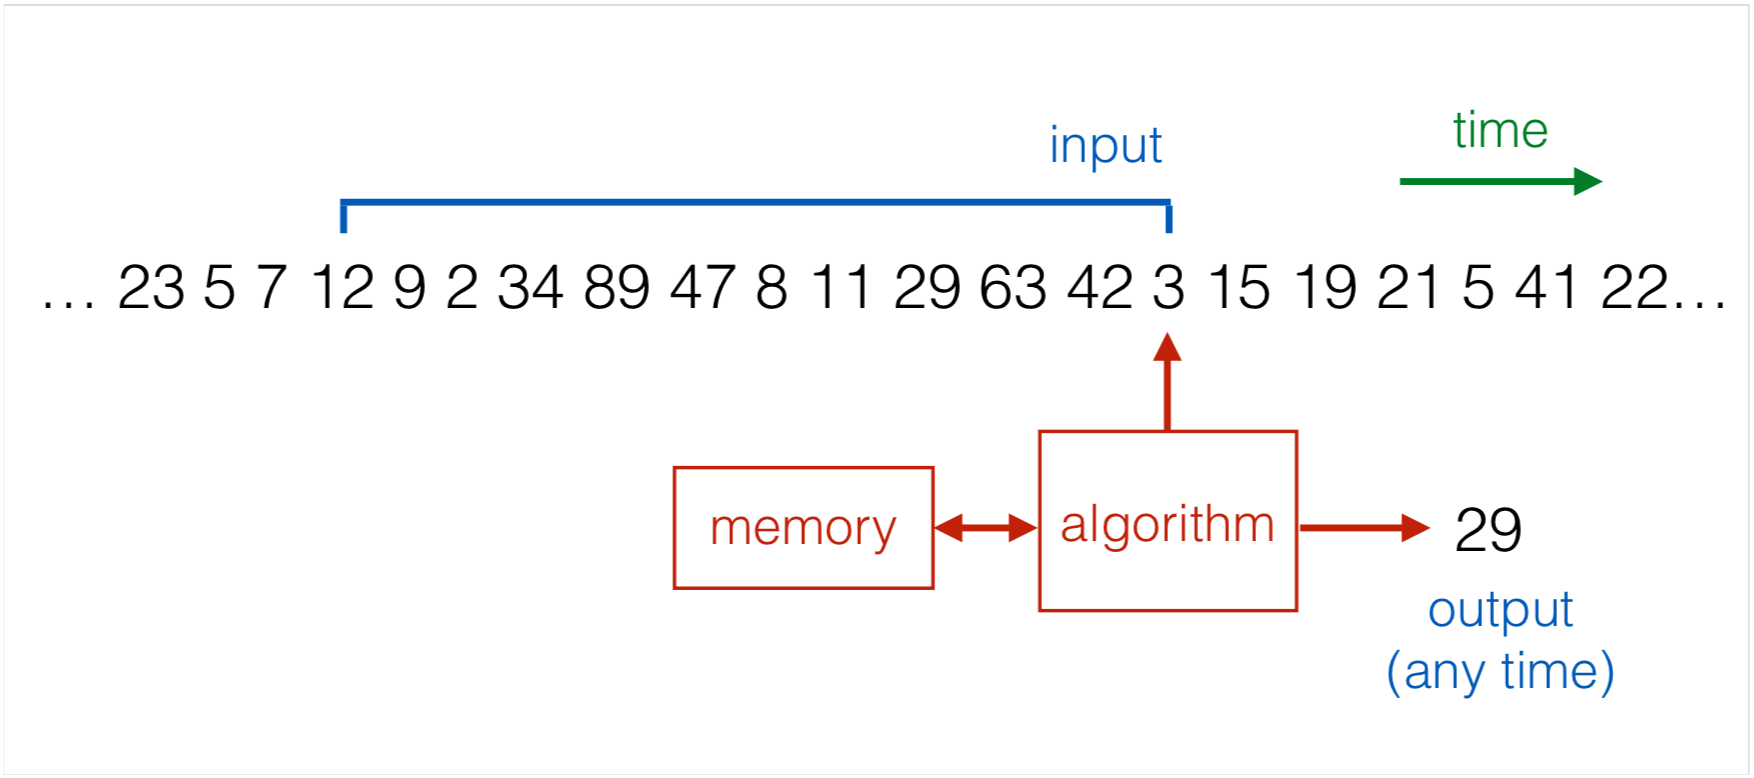
\includegraphics[width=12cm]{1_sliding_window.png}
          \captionof{figure}{Representation of sliding window: \textit{"CS-E4600 - slide set 7"}.}
        \end{center}

        Using the same logic and intuition we can argue that the \textit{priority sampling for sliding window} will use $\mathcal{O}(\log{w}\log{n})$, where $\log{w}$ is the length of the sliding window and $\log{n}$ is the space for numbers to be stored. The arguments for our prove are the criteria that:
        \begin{itemize}
          \item in any given window each item has equal chance to be selected as a random sample
          \item each removed element has a larger element proceeding it
          \item at any given point we expect the space efficiency $\mathcal{O}(w)$ with maximal elements
          \item and finally, maintaining list of maximal elements requires  $\mathcal{O}(\log{w})$ time
        \end{itemize}
      \item \textbf{Problem:} \textit{Reservoir algorithm for sampling 1 element in a data stream:}
        \begin{enumerate}
          \item \textbf{Question}: \textit{explain k-sample in a data stream is uniform:} \\
            The meaning of $k-sample$ in a data stream being uniform is: for randomly choosing a sample of $k$ items from a data stream, at any given time each element of the data stream have equal probability of being sampled.

          \item \textbf{Question}: \textit{value of the probability p:} \\
            The value of the probability will be the length of $k-sample$ divided by the value of how many elements at current time we have seen, $t$. Which is $\dfrac{k}{t}$.

          \item \textbf{Question}: \textit{prove that value of p gives uniform samples:} \\
            Let's suppose that our $k-sample$ has 5 elements. When sixth element arrives $i=6$ and $t=[1,2...6]$, each element is kept with the probability $\dfrac{5}{6}$, which is:
            \begin{align*}
              (1)(\frac{1}{6} + (\frac{5}{6})(\frac{4}{5})) = \frac{1}{6} + \frac{4}{6} = \frac{5}{6}
            \end{align*}
            when the seventh element arrives $i=7$ and $t=[1,2...7]$, the seventh element is kept with the probability $5/7$ and each of the previous $6$ elements are also kept with the same probability. Following that logic, we can prove by induction that when there are $n$ elements, each one is kept with the probability $5/n$. Consequently, our general notation will be:
            \begin{align*}
              P(k_{sample}|t_{elements\ seen}) = \frac{k}{t}
            \end{align*}

        \end{enumerate}

      \item \textbf{Problem:} \textit{Resort to sampling of good items:}
    \end{enumerate}
\end{document}
